\documentclass[11pt,a4paper]{article}

\usepackage[margin=2.5cm]{geometry}
\usepackage{amsmath,amssymb}
\usepackage{graphicx}
\usepackage{booktabs}
\usepackage{hyperref}
\usepackage{setspace}
\onehalfspacing

\title{BA-PPO: Blending Group-Relative and Critic-Based Advantages in Proximal Policy Optimization for Lunar Lander Control}

\author{[Student name] \\ [Student ID] \\ [Major] \\ [School / Department / Institute]}
\date{[Month X, Day X, 2026]}

\begin{document}

\maketitle

\begin{abstract}
Proximal Policy Optimization (PPO) estimates each action's advantage with a learned critic. Group Relative Policy Optimization (GRPO) removes the critic and scores each episode against other episodes that start from the same state. The episode-level score gives every step of an episode the same credit, which may be a weakness on long control tasks. We propose \emph{Blended Advantage PPO} (BA-PPO), which mixes the GRPO group score with the critic-based generalized advantage estimate (GAE) of PPO using an equal weight. We compare PPO, GRPO and BA-PPO on the LunarLander-v3 task at two minibatch sizes, with five test seeds and 2 million environment steps per run. Hyperparameters were chosen on separate tuning seeds. With minibatch size 64, BA-PPO reached an average final return of $256 \pm 14$, compared with $241 \pm 17$ for PPO and $167 \pm 60$ for GRPO. With minibatch size 512, BA-PPO was clearly ahead of both baselines. Against a tuned PPO, however, the difference is not statistically significant with five seeds. The blend weight was tested at three values on the tuning seeds, and the equal weight performed best.
\end{abstract}

\noindent\textbf{Keywords:} Reinforcement learning; Proximal policy optimization; Group relative policy optimization; Advantage estimation; Credit assignment; Lunar lander.

\section{Introduction}
\label{sec:intro}

Reinforcement learning (RL) trains an agent to choose actions that maximize long-term reward \cite{sutton2018rl}. Policy-gradient methods adjust a parameterized policy in the direction that increases expected reward \cite{williams1992reinforce,sutton1999policygradient}. Their practical success depends on how the gradient is estimated. The advantage of an action measures how much better it was than average in that state, and an accurate advantage estimate reduces the variance of the gradient while keeping it unbiased enough to learn from.

Proximal Policy Optimization (PPO) \cite{schulman2017ppo} is one of the most widely used policy-gradient methods. It limits how far each update can move the policy and estimates advantages with a learned value function (the critic) and generalized advantage estimation (GAE) \cite{schulman2016gae}. PPO builds on trust-region ideas \cite{schulman2015trpo}. Its reported performance also depends on implementation details that the original paper does not fully specify \cite{engstrom2020implementation}.

GRPO was introduced in the DeepSeekMath work \cite{shao2024deepseekmath} and used to train DeepSeek-R1 \cite{deepseekai2025r1}. It removes the critic. For each prompt, it samples a group of responses and scores each response relative to the group mean. A group baseline of this kind has been studied as a leave-one-out REINFORCE estimator \cite{ahmadian2024reinforce}. GRPO's per-episode score is simple and cheap, but it cannot tell which steps of an episode contributed to the outcome. Liu et al.\ \cite{liu2025r1zero} also show that GRPO's normalization introduces biases in how long responses are weighted.

On classical control tasks, a recent study reports that critic-free methods, including GRPO, trail PPO on long-horizon tasks and do well mainly on short ones \cite{marquesdeoliveira2025critics}. This raises the question we study here: can the episode-level group comparison be combined with the per-step critic so that the agent gets the benefit of both?

This report makes three contributions:
\begin{enumerate}
  \item BA-PPO, a minor extension of PPO. It adds a group-relative term to the advantage and keeps PPO's update rule unchanged.
  \item A controlled comparison of PPO, GRPO and BA-PPO on LunarLander-v3 under the same budget. Each method is tuned on separate seeds before the test runs, and the test uses five seeds per setting with significance tests.
  \item A test of the blend weight and an honest account of what the results do and do not show.
\end{enumerate}

\section{Problem Formulation}
\label{sec:problem}

We model the task as a Markov decision process (MDP) $\mathcal{M} = (\mathcal{S}, \mathcal{A}, P, r, \gamma)$, where $\mathcal{S}$ is the state space, $\mathcal{A}$ the action space, $P(s' \mid s, a)$ the transition kernel, $r(s,a)$ the reward and $\gamma \in [0,1)$ the discount factor. A stochastic policy $\pi_\theta(a \mid s)$ with parameters $\theta$ generates trajectories $\tau = (s_0, a_0, r_0, s_1, \dots, s_T)$. The goal is to maximize the expected discounted return
\begin{equation}
J(\theta) = \mathbb{E}_{\tau \sim \pi_\theta}\left[\sum_{t=0}^{T} \gamma^t r_t\right].
\label{eq:objective}
\end{equation}
Policy-gradient methods use the identity $\nabla_\theta J(\theta) = \mathbb{E}\left[\sum_t \nabla_\theta \log \pi_\theta(a_t \mid s_t)\, \hat{A}_t\right]$, where $\hat{A}_t$ estimates the advantage $A^{\pi}(s_t, a_t) = Q^{\pi}(s_t, a_t) - V^{\pi}(s_t)$. Any choice of $\hat{A}_t$ that does not depend on the action being evaluated keeps the gradient usable, but the choice strongly affects its variance and bias.

The problem has three difficulties that the methods below address in different ways:
\begin{itemize}
  \item \textbf{Credit assignment.} The reward at the end of a landing depends on many earlier actions \cite{pignatelli2024credit}. An estimate that gives all steps the same credit cannot separate useful actions from harmful ones within one episode.
  \item \textbf{Variance and sample cost.} A single episode is a noisy sample of the return. Critic-based estimates reduce variance but add a learned function whose errors can bias the update.
  \item \textbf{Sensitivity to implementation.} Small implementation choices can change the apparent ranking of methods, and results vary widely across random seeds \cite{engstrom2020implementation,henderson2018matters}.
\end{itemize}

LunarLander-v3 is a concrete instance of this problem. The observation $s_t \in \mathbb{R}^8$ contains the lander's position, velocity, angle, angular velocity and two leg-contact indicators. The action set is $\mathcal{A} = \{0, 1, 2, 3\}$ (do nothing, fire the left, main or right engine). A soft landing gives about $+100$, a crash gives $-100$, and each engine firing costs a small amount. A return of 200 or more is the standard criterion for solving the task. The episode ends when the lander lands, crashes, or leaves the view.

\section{Related Work}
\label{sec:related}

Policy-gradient methods began with REINFORCE \cite{williams1992reinforce}. Its gradient estimate is unbiased but has high variance. Sutton et al.\ \cite{sutton1999policygradient} gave the policy-gradient theorem for function approximation, and Schulman et al.\ \cite{schulman2015trpo} added a trust region to keep each update small. PPO \cite{schulman2017ppo} replaced the constrained optimization with a clipped objective that is simpler to implement. GAE \cite{schulman2016gae} gave the advantage estimator used by PPO and controls the bias--variance trade-off with the parameter $\lambda$. Deep value-based methods such as DQN \cite{mnih2015dqn} established the use of neural networks for RL on high-dimensional inputs, but they are not directly comparable to the policy-gradient methods studied here.

Critic-free alternatives have appeared recently. GRPO \cite{shao2024deepseekmath} scores each sample against a group of samples from the same prompt, and its use in DeepSeek-R1 \cite{deepseekai2025r1} drew wide attention. Ahmadian et al.\ \cite{ahmadian2024reinforce} showed that REINFORCE-style estimators with a leave-one-out baseline can compete with PPO for language-model alignment. Liu et al.\ \cite{liu2025r1zero} analyzed GRPO's normalization terms and proposed a corrected version. For classical control, Marques de Oliveira et al.\ \cite{marquesdeoliveira2025critics} found that critic-free methods, GRPO included, usually fall behind PPO on long-horizon tasks. Our study extends that comparison by combining both signals rather than choosing one.

The way methods are compared also matters. Henderson et al.\ \cite{henderson2018matters} showed that results across random seeds can differ widely and recommended significance tests. Agarwal et al.\ \cite{agarwal2021precipice} argued that point estimates from few runs are unreliable and recommended interval estimates. Engstrom et al.\ \cite{engstrom2020implementation} showed that implementation details can explain much of the reported gap between PPO and TRPO. Our experimental protocol follows these recommendations: separate tuning seeds, equal tuning budgets, five test seeds, and significance tests.

\section{Methods}
\label{sec:methods}

All three methods use the same actor network, the same critic network (when the method uses one), the same rollout procedure and the same clipped PPO update. Each network has two hidden layers of 64 units with $\tanh$ activations. The actor outputs a categorical distribution over the four actions. The methods differ only in how the advantage $\hat{A}_t$ is computed. This keeps the comparison controlled, and it means that BA-PPO's only change to PPO is the advantage term.

\subsection{Proximal Policy Optimization (PPO)}

Let $r_t(\theta) = \pi_\theta(a_t \mid s_t) / \pi_{\theta_{\text{old}}}(a_t \mid s_t)$ be the probability ratio between the new and old policies. PPO maximizes
\begin{equation}
L^{\text{clip}}(\theta) = \mathbb{E}_t\left[\min\left(r_t(\theta)\hat{A}_t,\; \text{clip}\left(r_t(\theta), 1-\epsilon, 1+\epsilon\right)\hat{A}_t\right)\right],
\label{eq:ppo}
\end{equation}
with $\epsilon = 0.2$. The advantage is estimated with GAE \cite{schulman2016gae}:
\begin{equation}
\hat{A}^{\text{GAE}}_t = \sum_{l=0}^{T-t-1} (\gamma\lambda)^l \delta_{t+l}, \qquad \delta_t = r_t + \gamma V(s_{t+1}) - V(s_t),
\label{eq:gae}
\end{equation}
with $\gamma = 0.99$ and $\lambda = 0.95$. The critic $V$ is trained by regression onto the GAE return targets. The advantages are normalized over each batch.

\subsection{Group Relative Policy Optimization (GRPO)}

GRPO \cite{shao2024deepseekmath} replaces the critic with a group baseline. For each start state, $G$ episodes are sampled under the same initial conditions. Let $R_i$ be the total reward of episode $i$. Its group-relative score is
\begin{equation}
\hat{A}^{\text{GRPO}}_i = \frac{R_i - \mathrm{mean}(R_1,\dots,R_G)}{\mathrm{std}(R_1,\dots,R_G) + 10^{-8}},
\label{eq:grpo}
\end{equation}
and each step $t$ of episode $i$ receives $\hat{A}_t = \hat{A}^{\text{GRPO}}_i$. We use $G = 8$. GRPO has no value function, so the value loss is not used. Because each step is averaged in the loss, longer episodes contribute more steps to the update. This is the behavior that \cite{liu2025r1zero} identify in GRPO's length normalization, and we keep it unchanged so that our implementation matches the standard form.

\subsection{Blended Advantage PPO (BA-PPO)}

BA-PPO combines the two signals. For step $t$ of episode $i$,
\begin{equation}
\hat{A}_t = \alpha\, \hat{A}^{\text{GRPO}}_i + (1-\alpha)\, \widetilde{A}^{\text{GAE}}_t,
\label{eq:bappo}
\end{equation}
where $\widetilde{A}^{\text{GAE}}_t$ is the GAE estimate normalized over the batch, and $\alpha = 0.5$. The critic is trained exactly as in PPO. When $\alpha = 0$, the method reduces to PPO. When $\alpha = 1$, the policy update uses only the group score.

The intuition is that the GRPO term provides an episode-level signal that is less affected by critic errors, while the GAE term provides the per-step credit that the group score lacks. The minor innovation is the blend itself, which costs one line of code relative to PPO and keeps PPO's stability mechanisms.

\subsection{Training settings}

Table~\ref{tab:settings} lists the settings shared by all methods. Each update collects about 4,096 environment steps, split into minibatches. Two minibatch sizes (512 and 64) were compared, and each method was run with both.

\begin{table}[h]
\centering
\caption{Training settings shared by PPO, GRPO and BA-PPO.}
\label{tab:settings}
\begin{tabular}{@{}ll@{}}
\toprule
Setting & Value \\
\midrule
Steps per update & 4,096 \\
Minibatch size & 512 or 64 (see Section~\ref{sec:results}) \\
Epochs per update & 4 \\
Clip $\epsilon$ & 0.2 \\
Learning rate (Adam) & $3\times10^{-4}$ \\
Discount $\gamma$ / GAE $\lambda$ & 0.99 / 0.95 \\
Entropy coefficient & 0.01 \\
Value loss coefficient & 0.5 (PPO and BA-PPO only) \\
Gradient norm clip & 0.5 \\
GRPO group size $G$ & 8 episodes per start state \\
BA-PPO blend weight $\alpha$ & 0.5 \\
Total environment steps & $2 \times 10^6$ \\
\bottomrule
\end{tabular}
\end{table}

\section{Software Architecture and Implementation}
\label{sec:software}

The implementation uses Python 3.12, PyTorch 2.15 (CPU) for the networks, Gymnasium 1.4 with Box2D for the environment \cite{towers2024gymnasium,brockman2016gym}, and NumPy and SciPy for analysis. The default settings are close to those of common reference implementations of PPO \cite{huang2022cleanrl,raffin2021sb3}. The code is publicly available at \url{https://github.com/Prolanter/ba-ppo-lunarlander}.

A single training file, \texttt{ppo\_grpo.py}, contains the shared code: the networks, the rollout loop, the three advantage calculations and the PPO update. Each method and setting also has a small wrapper in \texttt{experiments/}, so that any single experiment can be run on its own. \texttt{run\_all.py} runs all methods over all seeds in parallel. \texttt{tune.py} runs the tuning on separate seeds (100 and 101). \texttt{analyze.py} produces the learning curves and tables, and \texttt{stats.py} runs the significance tests. During training, each run writes live progress, which \texttt{monitor.py} shows as a terminal table, and TensorBoard logs of the learning curves.

Runs were executed on a laptop with an 8-core AMD Ryzen 9 processor and 16 GB of memory, with eight runs in parallel and two threads per run. The README in the repository gives the exact commands for each result.

\section{Data Description}
\label{sec:data}

The experiments use no external dataset. The data are the interactions between the agent and the environment, generated by the Gymnasium LunarLander-v3 simulator \cite{towers2024gymnasium,brockman2016gym}. The simulator is seeded, so each run is reproducible. CartPole-v1 was used only for short tests of the code and is not part of the reported results.

\section{Experimental Design}
\label{sec:design}

Hyperparameters were chosen on tuning seeds 100 and 101, separate from the five test seeds 0 to 4. Each method was tuned with the same three candidate settings: minibatch 512, minibatch 64, and a longer planning horizon ($\gamma = 0.999$, $\lambda = 0.98$). The planning-horizon setting has no effect on GRPO, which does not use GAE. Its results were identical to the minibatch-512 runs, so it was excluded from the choice. For each method, the best setting on the tuning seeds was then run on the test seeds. The reported score for each run is the mean return of its last 100 training episodes. Results are shown as mean $\pm$ sample standard deviation over seeds. Significance is assessed with Welch's $t$-test and the Mann--Whitney $U$ test.

\section{Experimental Results}
\label{sec:results}

\subsection{Tuning}

\begin{table}[h]
\centering
\caption{Tuning results on the separate tuning seeds (100 and 101). Each value is the mean of the last-100-episode return over the two seeds.}
\label{tab:tuning}
\begin{tabular}{@{}lccc@{}}
\toprule
Method & Minibatch 512 & Minibatch 64 & Planning horizon \\
\midrule
PPO & 140 & \textbf{251} & 120 \\
GRPO & 95 & \textbf{101} & 95 (identical to 512) \\
BA-PPO & 206 & \textbf{271} & 185 \\
\bottomrule
\end{tabular}
\end{table}

Minibatch size 64 was the best setting for all three methods, so it was used as the second setting in the main comparison. The difference for GRPO between 512 and 64 is small and within the noise of two seeds.

\subsection{Blend weight}

BA-PPO was tested with $\alpha = 0.25$, $0.5$ and $0.75$ at minibatch 64, on the tuning seeds. The averages were $186$, $271$ and $205$, respectively. The equal weight was best on both tuning seeds. Because it was already the default, no further test-seed runs were needed for this comparison.

\subsection{Test results}

Table~\ref{tab:main} gives the final returns over the five test seeds at both minibatch sizes.

\begin{table}[h]
\centering
\caption{Final return on test seeds 0 to 4 after 2 million steps (mean $\pm$ sample standard deviation). Steps to 200 is the mean over the seeds that reached it.}
\label{tab:main}
\begin{tabular}{@{}lcccc@{}}
\toprule
Method & Minibatch & Final return & Seeds reaching 200 & Steps to 200 \\
\midrule
PPO & 512 & $89 \pm 34$ & 0 of 5 & -- \\
GRPO & 512 & $129 \pm 44$ & 0 of 5 & -- \\
BA-PPO & 512 & $214 \pm 40$ & 4 of 5 & 1.03M \\
\midrule
PPO & 64 & $241 \pm 17$ & 5 of 5 & 1.16M \\
GRPO & 64 & $167 \pm 60$ & 4 of 5 & 0.90M \\
BA-PPO & 64 & $\mathbf{256 \pm 14}$ & 5 of 5 & \textbf{0.76M} \\
\bottomrule
\end{tabular}
\end{table}

Figures~\ref{fig:mb512} and \ref{fig:mb64} show the learning curves. Each curve is the mean over five seeds, and the shaded band is one standard deviation.

\begin{figure}[h]
\centering
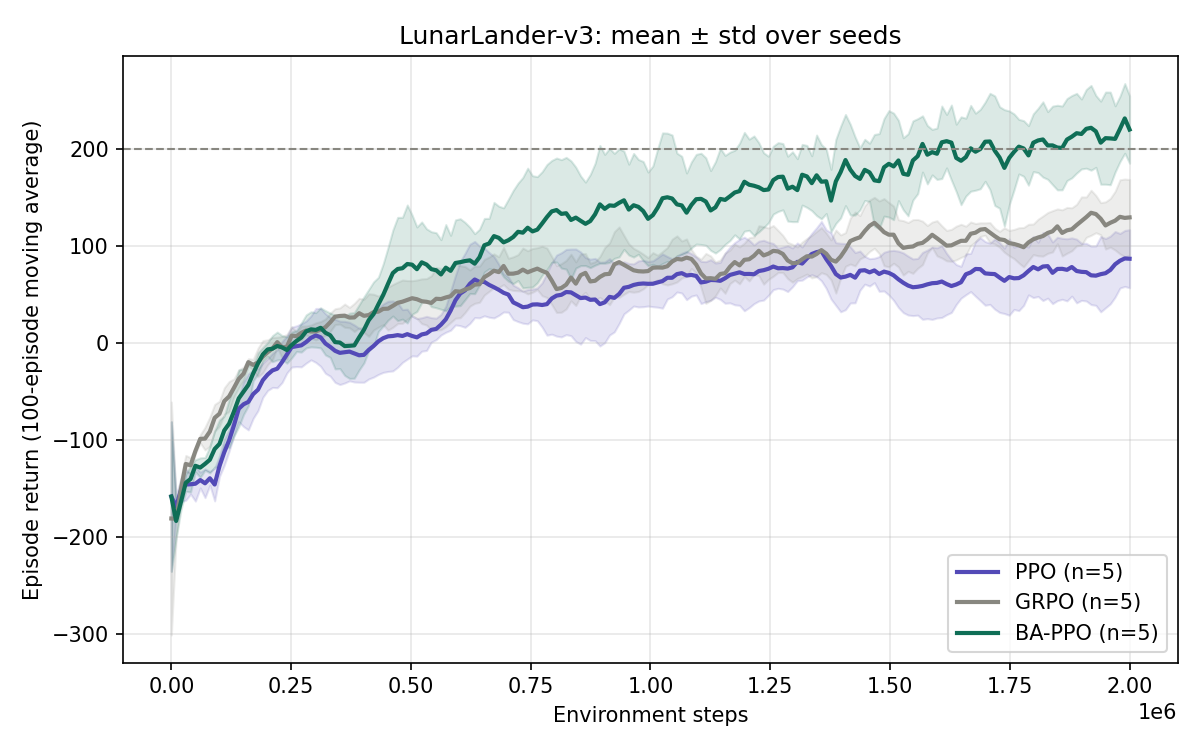
\includegraphics[width=0.85\linewidth]{figures/learning_curves_minibatch512.png}
\caption{Learning curves at minibatch 512 (mean $\pm$ 1 standard deviation over five seeds). The dashed line marks the solved score of 200.}
\label{fig:mb512}
\end{figure}

\begin{figure}[h]
\centering
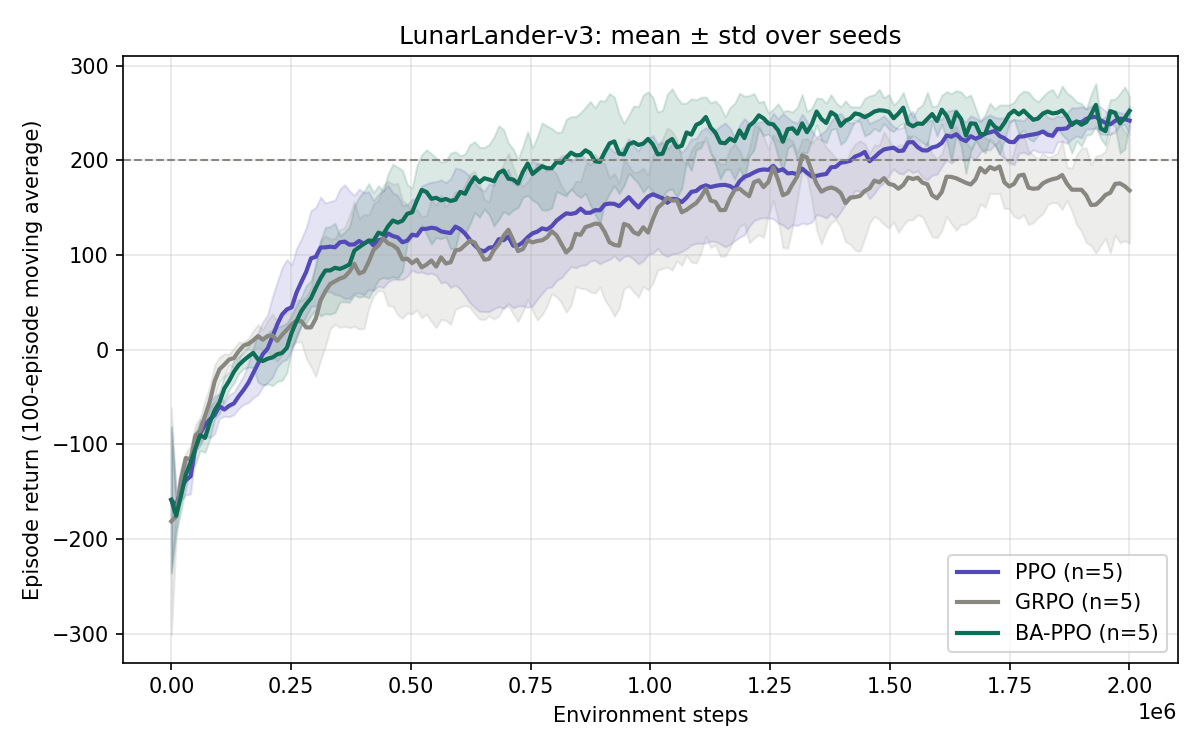
\includegraphics[width=0.85\linewidth]{figures/learning_curves_minibatch64.png}
\caption{Learning curves at minibatch 64 (mean $\pm$ 1 standard deviation over five seeds). The dashed line marks the solved score of 200.}
\label{fig:mb64}
\end{figure}

\subsection{Significance tests}

\begin{table}[h]
\centering
\caption{Pairwise comparisons of final returns over five test seeds. Both tests are two-sided.}
\label{tab:stats}
\begin{tabular}{@{}lrcc@{}}
\toprule
Comparison & Difference & Welch $p$ & Mann--Whitney $p$ \\
\midrule
\multicolumn{4}{l}{\emph{Minibatch 512}} \\
BA-PPO vs PPO & $+125$ & 0.001 & 0.008 \\
BA-PPO vs GRPO & $+85$ & 0.013 & 0.032 \\
GRPO vs PPO & $+41$ & 0.147 & 0.222 \\
\midrule
\multicolumn{4}{l}{\emph{Minibatch 64}} \\
BA-PPO vs PPO & $+15$ & 0.172 & 0.310 \\
BA-PPO vs GRPO & $+90$ & 0.028 & 0.056 \\
GRPO vs PPO & $-74$ & 0.049 & 0.095 \\
\bottomrule
\end{tabular}
\end{table}

\subsection{Discussion}

At minibatch 512, BA-PPO learns faster and more reliably than both baselines, and it is the only method that reached the solved score on most seeds. At minibatch 64, all three methods improve substantially, so the minibatch size matters a great deal for PPO. BA-PPO has the highest mean return and the lowest spread across seeds. It also reaches the solved score on every seed in the fewest steps on average. Its lead over the tuned PPO, however, is about 15 points, and it is not statistically significant with five seeds.

These findings are consistent with the earlier study of critic-free methods \cite{marquesdeoliveira2025critics}. Once the tuning is fair, GRPO trails PPO on this long-horizon task, and the gap is large enough to be significant. BA-PPO recovers the advantage of GRPO's group signal while keeping the critic, which the earlier study identifies as necessary for long horizons. The minibatch-512 results also show that the untuned PPO baseline can be much weaker than a tuned one. Comparisons that tune only the proposed method would therefore overstate its advantage, and this is why every method was tuned in the same way.

Several limitations apply. With five test seeds, the confidence in the differences is limited, and the interval estimates recommended by Agarwal et al.\ \cite{agarwal2021precipice} would be wider than our standard deviations suggest. The blend weight was tested at only three values on two tuning seeds. Learning rate, clipping, epochs and entropy weight were fixed for all methods, so other settings might change the ranking. The GRPO group size $G = 8$ was not varied, although the earlier study found that smaller groups can perform better. Wall-clock times are not directly comparable, because the runs shared the processor. Scores are returns from training episodes, which include the agent's random exploration.

\section{Conclusion}
\label{sec:conclusion}

We proposed BA-PPO, which blends the GRPO group-relative advantage with the PPO critic-based advantage. On LunarLander-v3, BA-PPO outperformed PPO and GRPO under the same budget with minibatch size 512, and it had the highest mean return and the most consistent results with minibatch size 64. The margin over a tuned PPO was not statistically significant with five seeds. An equal blend weight gave the best result among the three values tested. Future work should test more seeds, tune the learning rate and the blend weight for each method, vary the GRPO group size, and examine tasks with longer horizons, where the credit-assignment argument for blending should matter most.

\bibliographystyle{ieeetr}
\bibliography{references}

\end{document}
